
\documentclass[conference,a4paper,american,russian]{IEEEtran}
\usepackage{listings}
\usepackage{tikz}
\usepackage{amsmath,amssymb,amsfonts}
\usepackage{algorithmic}
\usepackage{graphicx}
\usepackage[T2A]{fontenc}
\usepackage[utf8]{inputenc}
\usepackage{babel}
\usepackage{hyperref}
\usepackage{balance}

\def\IEEEkeywordsname{Ключевые понятия}

\renewcommand{\sfdefault}{cmss}
\renewcommand{\rmdefault}{cmr}
\renewcommand{\ttdefault}{cmt}

\newcommand{\miniKanren}{\textsc{miniKanren}}
\newcommand{\mercury}{\textsc{Mercury}}
\newcommand{\haskell}{\textsc{Haskell}}
\newcommand{\prolog}{\textsc{Prolog}}
\newcommand{\scheme}{\textsc{Scheme}}
\newcommand{\logen}{\textsc{LOGEN}}

\newcommand{\github}{\textsc{GitHub}}

\lstset{mathescape=true}

\begin{document}


\title{Анализ времени связывания для реляционных программ}

\author{
\IEEEauthorblockN{Ирина Артемьева}
\textit{Университет ИТМО} \\
Санкт-Петербург, Россия \\
irinapluralia@gmail.com
\and
\IEEEauthorblockN{Екатерина Вербицкая}
\textit{JetBrains Research}\\
Санкт-Петербург, Россия \\
kajigor@gmail.com
}


\maketitle

\begin{abstract}
Программы в парадигме реляционного программирования представляют собой математические отношения.
Программы-отношения можно исполнять в различных направлениях: зафиксировав часть аргументов программы, находить значение остальных.
Не всегда исполнение программы в заданном направлении эффективно. 
Одним из способов улучшения производительности является трансляция реляционных программ в функциональные. 
Для генерации функции по отношению необходимо определить порядок связывания имен в программе с учётом заданного направления.
Для этого традиционно применяется анализ времени связывания, однако для реляционных языков ранее его разработано не было.
В статье мы предлагаем алгоритм анализа времени связывания для языка реляционного программирования \miniKanren{}. 
\end{abstract}

\begin{IEEEkeywords}
Реляционное программирование, анализ времени связывания, статический анализ
\end{IEEEkeywords}

\section{Введение}

Реляционное программирование --- парадигма, в которой любая программа описывает математическое отношение на её аргументах. 
Имея программу-отношение, можно выполнять запросы: указывая некоторые известные аргументы, получать значения остальных.
Например, $add^o \subseteq Int \times Int \times Int$ описывает отношение, третий аргумент которого является суммой первых двух. 
Рассмотрим возможные направления вычисления этого отношения (здесь и далее искомый аргумент будем обозначать знаком ``$?$'').
Выполнение отношения $add^o  \ x \ y \ ?$ с зафиксированными (входными) первым и вторым аргументом найдет их сумму, а $add^o \ ? \ y \ z$ найдет такие числа, которые в сумме с $y$ дадут $z$. 
Также можно найти одновременно значения нескольких аргументов: $add^o \ ? \ ? \ z$ найдет такие пары чисел, что в сумме они равны $z$, а $add^o \ ? \ ? \ ?$ перечислит все тройки из отношения. 

Таким образом, мы можем говорить о выборе \textit{направления} вычисления. 
Часто при написании программы подразумевается конкретное направление, называемое \textit{прямым} (например, $add^o  \ x \ y \ ?$), все остальные направления обычно называются \textit{обратными}. 
Возможность выполнения в различных направлениях --- основное преимущество реляционного программирования. 
Это своеобразный шаг к декларативности: достаточно написать одну программу для получения множества целевых функций. 

Реляционному программированию родственно логическое, представленное такими языками, как \prolog{} и \mercury{}\footnote{Официальный сайт языка \mercury{}: \url{https://mercurylang.org/}, дата последнего посещения: 15.02.2020}~\cite{SOMOGYI199617}.
Основным представителем парадигмы реляционного программирования является семейство интерпретируемых языков \miniKanren{}\footnote{Официальный сайт языка \miniKanren{}: \url{http://minikanren.org/}, дата последнего посещения: 15.02.2020}.
Языки семейства \miniKanren{} компактны и встраиваются в языки общего назначения, за счёт чего их проще использовать в  проектах. 
Для встраивания достаточно реализовать интерпретатор языка \miniKanren{}: ядро языка, реализованное на \scheme{} занимает не более, чем 40 строк~\cite{hemann2013ukanren}.
Помимо этого, \miniKanren{} реализует полный поиск со стратегией interleaving, поэтому любая программа, написанная на нем, найдет все существующие ответы, в то время как \prolog{} может никогда не завершить поиск. 
В этой статье мы будем говорить про \miniKanren{}.

Возможность выполнения программ на \miniKanren{} в различных направлениях позволяет решать задачи поиска посредством решения задачи распознавания~\cite{lozov2019relational}.
Так, имея интерпретатор языка, можно решать задачу синтеза программ на этом языке по набору тестов~\cite{byrd2017unified}; имея функцию, проверяющую, что некоторая последовательность вершин в графе формирует путь с желаемыми свойствами, получать генератор таких путей и так далее. 
$N$-местную функцию-распознаватель, реализованную на некотором языке программирования, можно автоматически транслировать на \miniKanren{}, получив $N+1$-местное отношение, связывающее аргументы функции с булевым значением~\cite{lozov2019relational} (истина соответствует успешному распознаванию). 
Зафиксировав значение $N+1$-ого булевого аргумента, можно выполнять поиск. 
Ценность такого подхода в его простоте: решение задачи поиска всегда труднее, чем реализация распознавателя. 

К сожалению, выполнение отношения в обратном направлении обычно крайне не эффективно. 
В~\cite{lozov2019relational} для решения этой проблемы используется специализация. 
В статье показано, что специализация приводит к существенному приросту скорости работы программы.
Однако чтобы избавиться от всех накладных расходов, связанных с интерпретацией программы, необходим Джонс-оптимальный специализатор~\cite{jones1993partial}. 
К сожалению, реализация такого специализатора --- нетривиальная задача.

В данное время авторами ведется работа над альтернативным подходом улучшения производительности программы в заданном направлении. 
Для этого по отношению с фиксированным направлением генерируется функция на функциональном языке программирования \haskell{}. 
Таким образом можно избежать затрат на интерпретацию. 
Особенностью реляционного программирования является отсутствие строго порядка исполнения программы: особенно сильно он может отличаться для разных направлений.
Это затрудняет трансляцию в функциональные языки программирования. 
Для успешной трансляции необходимо определить порядок исполнения программ с учётом направления. 
Для решения такой задачи используется \textit{анализ времени связывания} (binding time analysis). 
Функционально-логический язык программирования \mercury{} использует анализ времени связывания как шаг компиляции~\cite{vanhoof2004binding}, однако для реляционных языков такой анализ ранее не применялся.
В данной статье мы представляем алгоритм времени связывания для реляционного программирования. 

В разделе~\ref{miniKanren} мы описываем язык \miniKanren{}, используемый в статье.
Раздел~\ref{translator} описывает схему его трансляции в функциональный язык и возникающие при этом трудности.
Алгоритм анализа времени связывания для \miniKanren{} приведен в разделе~\ref{bta}. 
Обзор литературы --- в разделе~\ref{related}.
В заключении (раздел ~\ref{conclusion}) подведены итоги и описаны планы на дальнейшую работу. 

\section{Язык программирования \miniKanren{}}\label{miniKanren}

Семейство языков \miniKanren{} дало рождение парадигме реляционного программирования. 
Это минималистичные языки, встраиваемые в языки программирования общего назначения. 
Помимо простоты использования при разработке конечных приложений, \miniKanren{} реализует полный поиск: все существующие решения будут найдены, пусть и за длительное время.
Классический представитель родственной парадигмы логического программирования \prolog{} этим свойством не обладает: исполнение программы может не завершиться, даже если не все решения были вычислены. 
Незавершаемость программ на \prolog{} --- свойство стратегии поиска решения.
Для устранения потенциальной нетерминируемости используются нереляционные конструкции, такие как cut. 
Эта особенность существенно усложняет и часто делает невозможным исполнение в обратном направлении. 
Язык \miniKanren{} же является чистым: все языковые конструкции обратимы. 

Программа на \miniKanren{} состоит из набора определений отношений и цели. 
Определение имеет имя, список аргументов и тело.
Тело отношения является \textit{целью}, которая может содержать \textit{унификацию термов} и \textit{вызовы отношений}, скомбинированные при помощи \textit{дизъюнкций} и \textit{конъюнкций}. 
\textit{Терм} представляет собой или \textit{переменную}, или \textit{конструктор} с именем и списком подтермов. 
Свободные переменные вводятся в область видимости при помощи конструкции $\underline{fresh}$. 
Абстрактный синтаксис языка приведен ниже:
\begin{align*}
  Goal &: Goal \vee Goal \\
       &\mid Goal \wedge Goal \\
       &\mid Term \equiv Term \\
       &\mid \underline{call} \ Name \ [Term] \\
       &\mid \underline{fresh} \ [Var] \ Goal \\
  Term &: Var \\ 
       &\mid \underline{cons} \ Name \ [Term]
\end{align*}

Пример программы на языке \miniKanren{}, связывающей три списка, где третий является конкатенацией первых двух, приведен на рис.~\ref{lst:appendoDEF}. 
Для краткости $[]$ заменяет пустой список ($\underline{cons} \ Nil \ []$); $h : t$ обозначает список с головой $h$ и хвостом $t$ ($\underline{cons} \ Cons \ [h, t]$), а $[x_0, x_1, \dots, x_n]$ --- список с элементами $x_0, x_1, \dots, x_n$. 
Вызов отношения $\underline{call} \ relation \ [t_0, \dots t_k]$ записывается как $relation \ t_0 \dots \ t_k$.

\begin{figure}[h!]
  \begin{center}
  \begin{minipage}{0.3\textwidth}
  \begin{lstlisting}[language=Haskell, frame=single, numbers=left,numberstyle=\small, escapechar=|]
  $append^o$ x y z =
    (x $\equiv$ [] $\wedge$ y $\equiv$ z) $\vee$ |\label{line:ma2}|
    (fresh [h, t, r] (
        x $\equiv$ h : t $\wedge$ |\label{line:ma4}|
        z $\equiv$ h : r $\wedge$ |\label{line:ma5}|
        $append^o$ t y r |\label{line:ma6}|
    ))
    \end{lstlisting}
  \end{minipage}
  \end{center}
  \caption{Пример программы на \miniKanren{}}
  \label{lst:appendoDEF}
\end{figure}

Исполнение этого отношения в прямом направлении на двух заданных списках $append^o \ [1,2] \ [3] \ ?$ вернёт их конкатенацию $[1,2,3]$.
Если исполнить его в обратном направлении, оставив первые два аргумента неизвестными, мы получим все возможные разбиения данного списка на два: результатом $append^o \ ? \ ? \ [1,2,3]$ является множество пар $\{([],[1,2,3]), ([1], [2,3]), ([1,2], [3]), ([1,2,3], [])\}$.

\section{Трансляция в функциональный язык}\label{translator}

В этом разделе мы кратко опишем разрабатываемую авторами трансляцию \miniKanren{} в функциональный язык программирования, чтобы продемонстрировать, на решение каких проблем нацелен анализ времени связывания.
Мы будем использовать \haskell{} в качестве целевого языка. 

Отношение, выполненное в заданном направлении, можно рассматривать как функцию из известных аргументов в неизвестные. 
Например, отношение $append^o$, выполненное в прямом направлении ($append^o \ x \ y \ ?$), соответствует функции конкатенации списков $x$ и $y$. 

Отношение $append^o$ состоит из двух дизъюнктов. 
Первый дизъюнкт означает, что если $x$ является пустым списком, то $y$ совпадает с $z$. 
Второй дизъюнкт означает, что $x$ и $z$ являются списками, начинающимися с одного и того же элемента, при этом хвостом $z$ является результат конкатенации хвоста списка $x$ со списком $y$. 
Унификация с участием неизвестной переменной $z$ указывает на то, \emph{как} вычислить её значение, в то время как унификация  известной переменной $x$ --- \emph{при каком условии}.

Автоматическая трансляция $append^o$ в прямом направлении создаст функцию, приведенную на листинге~\ref{lst:appendoFWD}. 
В двух уравнениях первая переменная сопоставляется с образцом. 
В первом случае мы сразу возвращаем второй список как результат, в то время как во втором необходимо осуществить рекурсивный вызов построенной функции. 

\begin{figure}[h!]
  \begin{center}
  \begin{minipage}{0.35\textwidth}
  \begin{lstlisting}[language=Haskell, frame=single, numbers=left,numberstyle=\small, firstnumber=8, escapechar=|]
  $append^o$ :: [a] $\to$ [a] $\to$ [a]
  $append^o$ [] y = y
  $append^o$ (h : t) y =
    let r = $append^o$ t y in 
    h : r 
  \end{lstlisting}
  \end{minipage}
  \end{center}
  \caption{Результат трансляции $append^o \ x \ y \ ?$}
  \label{lst:appendoFWD}
\end{figure}

Не всегда результатом выполнения отношения является единственный ответ.
Например, при выполнении отношения $append^o$ в обратном направлении ($append^o \ ? \ ? \ z$), \miniKanren{} вычислит \emph{все} возможные \emph{пары} списков, дающие при конкатенации~$z$. 
В~общем случае отношению $R \subseteq X_0 \times \dots \times X_n$, с известными аргументами $X_{i_0}, \dots X_{i_k}$, и неизвестными $X_{j_0}, \dots X_{j_l}$, соответствует функция, возвращающая список результатов $F : X_{i_0} \to \dots \to X_{i_k} \to [X_{j_0} \times \dots \times X_{j_l}]$. 

Любое отношение можно преобразовать в \emph{нормальную форму} (для упрощения повествования мы будем считать, что все цели нормализованы). 
\emph{Нормальной формой} будем называть дизъюнкцию конъюнкций вызовов отношений или унификаций термов, в которой все свободные переменные введены в область видимости в самом начале:
\begin{align*}
  Goal  &: \underline{fresh} \ [Name] \ (\bigvee \bigwedge Goal') \\
  Goal' &: \underline{call} \ Name \ [Term] \\
        &\mid Term \equiv Term 
\end{align*}

Транслятор строит одну функцию для каждого дизъюнкта. 
Дизъюнкты в программе на \miniKanren{} независимы, то есть все ответы из каждого дизъюнкта объединяются для получения результата выполнения отношения. 
Для отношения создается функция, конкатенирующая результаты применения функций, построенных для отдельных дизъюнктов. 

Пример трансляции $append^o \ ? \ ? \ z$ приведен в листинге~\ref{lst:appendoBWD}.  
Унификации неизвестных переменных (например $x \equiv []$ и $x \equiv h : t$) при трансляции преобразуются в let-связывания (строки~\ref{line:h2a2} и~\ref{line:h2a10}). 
Рекурсивные вызовы отношений транслируются в рекурсивные вызовы функций, построенных в заданном направлении (см. строку~\ref{line:h2a9}).
Стоит обратить внимание, что рекурсивно вызывается функция $append^o$, построенная по всему отношению.
Мы используем do-нотацию языка \haskell{}\footnote{Описание do-нотации языка \haskell{}: \url{https://en.wikibooks.org/wiki/Haskell/do\_notation}, дата последнего посещения: 15.02.2020}.
Связывание в строке~\ref{line:h2a9} означает, что результат будет вычислен для каждого элемента списка, полученного из рекурсивного вызова функции.

\begin{figure}[h!]
  \begin{center}
  \begin{minipage}{0.4\textwidth}
    \begin{lstlisting}[language=Haskell, frame=single, numbers=left, numberstyle=\small, firstnumber=13, escapechar=|]
  $append^o$ :: [a] $\to$ [([a], [a])]
  $append^o$ x = $append^o_1$ x ++ $append^o_2$ x
    where
      $append^o_1$ y = do
        let x = []          |\label{line:h2a2}|
        return (x, y)
      $append^o_1$ _ = []
      
      $append^o_2$ (h : r) = do
        (t, y) $\leftarrow$ $append^o$ r |\label{line:h2a9}|
        let x = h : t       |\label{line:h2a10}|
        return (x, y)
      $append^o_2$ _ = []
      \end{lstlisting}
  \end{minipage}
  \end{center}
  \caption{Результат трансляции $append^o \ ? \ ? \ z$ }
  \label{lst:appendoBWD}
\end{figure}

Нетрудно заметить, что порядок вычислений в функциях нередко не совпадает с порядком конъюнктов в исходном отношении. 
Например, рекурсивный вызов отношения $append^o$ производится в последнем конъюнкте (см. рис.~\ref{lst:appendoDEF}, строка~\ref{line:ma6}), в то время как в функциях выполняется в первую очередь. 
Если отношение вызывает более одного отношения, то необходимо не только определить порядок, в котором необходимо вызывать функции в результате трансляции, но и в каком направлении это делать. 
Примером может служить отношение $revers^o$ (см. листинг~\ref{lst:reversoDEF}), связывающий список со списком его элементов в обратном порядке.
Это отношение имеет рекурсивный вызов, а также вызов отношения $append^o$. 
Порядок вызовов здесь влияет на направления функций, построенных по этим отношениям.
Выбранные направления также могут влиять на то, в каком порядке необходимо вызывать функции. 
Использование монадических вычислений и do-нотации вынуждает нас заранее определять порядок, в котором будут осуществляться вызовы функций. 

\begin{figure}[h!]
  \begin{center}
  \begin{minipage}{0.35\textwidth}
  \begin{lstlisting}[language=Haskell, frame=single, numbers=left,numberstyle=\small, firstnumber=26,escapechar=|]
  $revers^o$ xs sx =
    (xs $\equiv$ [] $\wedge$ sx $\equiv$ []) $\vee$
    (fresh [h, ts, st] (
        x $\equiv$ h : ts $\wedge$
        $revers^o$ ts st $\wedge$
        $append^o$ st [h] sx
    ))
    \end{lstlisting}
  \end{minipage}
  \end{center}
  \caption{Отношение $revers^o$}
  \label{lst:reversoDEF}
\end{figure}

Эти особенности диктуют необходимость использования некоторого статического анализа, позволяющего упорядочить вычисления в заданном направлении. 
Анализ времени связывания часто используется при построении offline-специализаторов языков программирования. 
Его задачей является определить, являются ли данные, используемые в программах, статическими (известными заранее) или динамическими (известными только во время вычисления).
Использование анализа времени связывания при функциональной трансляции может также определить порядок вычисления, а по нему --- направления, в которых необходимо транслировать используемые отношения. 

\section{Анализ времени связывания для \miniKanren{}}\label{bta}

Цель анализа времени связывания --- указать порядок, в котором имена связываются со значениями.
Алгоритм принимает на вход программу на \miniKanren{} и данные о том, какие переменные считаются входными. 
В результате работы алгоритма каждой переменной ставится в соответствие положительное число, обозначающее время связывания этой переменной.
Мы будем называть процесс подбора чисел \emph{аннотированием}.

Если о переменной ничего неизвестно, она аннотируется $Undef$; иначе указывается время связывания: целое положительное число.
В начале работы алгоритма известными являются переменными, указанные как входные --- они аннотируются числом $0$.
Если переменная унифицируется с константой (термом, не содержащим свободных переменных), то мы считаем $1$ её временем связывания. 
Если переменная унифицируется с термом, каждая свободная переменная которого аннотирована, мы аннотируем эту переменную числом $1+n$, где $n$ --- максимальная аннотация свободных переменных терма. 
Таким образом мы распространяем информацию о времени связывания на непроаннотированные переменные.

На аннотациях имеется порядок: естественный порядок на положительных числах, при этом $Undef$ считается меньше любой числовой аннотации.
Ранее проаннотированная переменная может получить другую аннотацию, если появилась какая-то новая информация о её времени связывания.
При этом аннотация никогда не заменяется на меньшую. 

\begin{figure}[htbp]
  \centering
  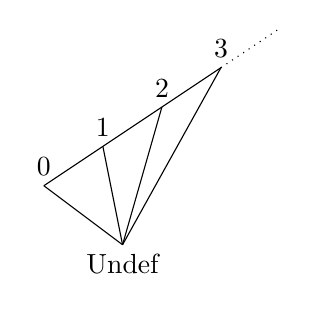
\begin{tikzpicture}
    \draw (1,0) node[below] {Undef};
    \draw (0,.75) node[above] {0};
    \draw (.75,1.25) node[above] {1};
    \draw (1.5,1.75) node[above] {2};
    \draw (2.25,2.25) node[above] {3};
    \draw (1,0) -- (0,.75);
    \draw (1,0) -- (.75,1.25);
    \draw (1,0) -- (1.5,1.75);
    \draw (1,0) -- (2.25,2.25);
    \draw (0,.75) -- (2.25,2.25);
    \draw[dotted] (2.25,2.25) -- (3,2.75);
  \end{tikzpicture}
  \caption{Полурешетка на аннотациях}
  \label{fig:image}
\end{figure}

\subsection{Алгоритм анализа времени связывания}

Реализация разработанного алгоритма доступна на сайте \github{}\footnote{Исходный код алгоритма аннотирования: \url{https://github.com/Pluralia/uKanren\_translator}, дата последнего посещения: 15.02.2020}. Ниже приведено описание алгоритма.

Входные данные алгоритма: программа на \miniKanren{} (цель) и список входных переменных.
Выходные данные --- пара из проаннотированной нормализованной (приведенной к дизъюнктивной нормальной форме) цели и списка проаннотированных определений отношений, вызываемых целью. 
Мы будем называть этот список \emph{стеком вызова}, потому что в нем будут находиться вызываемые отношения.

При инициализации алгоритма выполняются следующие действия: 
\begin{itemize}
    \item все $fresh$-переменные уникально переименовываются, чтобы избежать перекрытия имен;
    \item цель приводится в дизъюнктивную нормальную форму;
    \item все входные переменные аннотируются $0$;
    \item создается пустой стек вызовов.
\end{itemize}

Каждый раз при обработке вызова отношения анализуруется его тело, при этом: 
\begin{itemize}
    \item $fresh$-переменные уникально переименовываются;
    \item цель приводится в нормальную форму;
    \item производится первичное аннотирование цели данными о входных переменных.
\end{itemize}

Аннотация цели осуществляется итеративно, пока не будет достигнута неподвижная точка функции, описывающей шаг аннотирования. 
За один шаг мы аннотируем либо одну унификацию, либо один вызов отношения. 
Для аннотации цели в нормальной форме необходимо проаннотировать все её дизъюнкты. 
Аннотации переменных в дизъюнкте должны согласовываться: одна и та же переменная в конъюнктах одного дизъюнкта должна иметь одну и ту же аннотацию.
Конъюнкты аннотируются в заранее определенном порядке. 
Сначала мы аннотируем унификации, а затем вызовы отношений. 
Каждый раз при аннотации новой переменной необходимо установить ту же аннотацию всем другим вхождениям этой переменной в дизъюнкте. 

При аннотировании унификаций возможны следующие случаи. 
Здесь и далее аннотация переменной указывается в верхнем индексе.
\begin{itemize}
    \item Унификация имеет вид $x^{Undef} \equiv t[y_0^{i_0}, \dots, y_k^{i_k}]$, то есть переменная, имеющая аннотацию $Undef$, унифицируется с термом $t$ со свободными переменными $y_j^{i_j}$ с целочисленными аннотациями $i_j$. В~таком случае переменной $x$ необходимо присвоить аннотацию $n + 1$, где $n = max \{ i_0, \dots i_k\}$.
    \item Переменная, аннотированная числом, унифицируется с термом: $x^{n} \equiv t[y_0^{i_0}, \dots, y_k^{i_k}]$; некоторые свободные переменные терма проаннотированы $Undef$.
    Тогда всем переменным $y_j^{Undef}$ присваивается аннотация $n+1$.
    \item Оба унифицируемых терма --- конструкторы: $\underline{cons} \ Name \ [t_0^{i_0}, \dots, t_k^{i_k}] \equiv \underline{cons} \ Name \ [s_0^{j_0}, \dots, s_k^{j_k}]$.
    В этом случае имена конструкторов должны быть одинаковыми, а количество термов --- совпадать, иначе такие термы унифицировать не удастся.
    Такая унификация эквивалентна конъюнкции унификаций вида $t_l^{i_l} \equiv s_l^{j_l}$, каждую из которых следует анализировать в соответствии с одним из перечисленных случаев.  
    \item Остальные случаи симметричны.
\end{itemize}

Помимо унификации конъюнкт может быть вызовом некоторого отношения на частично проаннотированных термах. 
Для аннотации вызова мы рассматриваем тело соответствующего отношения и аннотируем его. 
Для избежания повторного аннотирования информация о ранее проаннотированных в конкретных направлениях отношениях сохраняется в стеке вызовов.
Если частично определенное направление текущего вызова согласовано с ранее проаннотированным, анализировать его не нужно.  
Два направления назовем \emph{согласованными}, если при попарном сравнении аннотаций их аргументов аннотации одного направления будут всегда не меньше соответствующих аннотаций другого.

Для иллюстрации понятия согласованных направлений рассмотрим следующие примеры. 
Пусть есть отношение $r^o$ с частично определенными направлениями: $r^o \ x^0 \ y^0 \ z^{Undef}$ и $r^o \ x^1 \ y^0 \ z^{Undef}$.
Они являются согласованными, так как аннотации переменной $x$ упорядочены правильно ($0 < 1$), а для $y$ и $z$ аннотации совпадают.
При этом, направление $r^o \ x^3 \ y^2 \ z^0$ не согласовано с направлением $r^o \ x^0 \ y^0 \ z^2$, так как аннотации $x$ и $y$ больше в первом направлении, а  $z$ --- во втором.

При аннотации вызовов отношений возможны следующие случаи. 
\begin{itemize}
    \item Переменные всех аргументов проаннотированы $Undef$. В этом случае для аннотирования не достаточно информации, поэтому следует перейти к аннотации следующего конъюнкта. 
    \item Вызов полностью проаннотирован, то есть аннотация всех переменных --- числа. Здесь дальнейшая аннотация не требуется.
    \item Вызов с таким именем и согласованным направлением уже есть в стеке вызовов --- заменить $Undef$-аннотации переменных на $n+1$, где $n$ --- максимальная аннотация переменных согласованного направления.
    \item Вызова с таким именем и направлением нет в стеке вызовов.
    В этом случае мы сначала добавляем его и направление в стек вызовов. 
    Затем аннотируем тело вызываемого отношения с учётом обновленного стека. 
    По завершении аннотации добавляем в стек проаннотированную цель.
\end{itemize}

Существуют отношения, точная аннотация которых не возможна без вмешательства человека или полного перебора возникающих вариантов. 
В таких отношениях некоторые переменные используются только в отношениях, не участвуя в унификациях.
Пример такого отношения приведен в листинге~\ref{lst:reloDEF}.
Пусть $y$ --- входная переменная.
В этом случае порядок вычисления вызовов $f^o$ и $h^o$ не зависит друг от друга, но зависит от направления вычисления $g^o$.
Оно не может вычисляться до вычисления $f^o$ и $h^o$ (неизвестны входные переменные), но может вычисляться между ними (в прямом или обратном порядке) или после (выполнять роль предиката).

\begin{figure}[h!]
  \begin{center}
  \begin{minipage}{0.18\textwidth}
  \begin{lstlisting}[language=Haskell, frame=single, numbers=left,numberstyle=\small, firstnumber=33, escapechar=|]
  $rel^o$ x y z =
    $f^o$ x y $\vee$
    $h^o$ z y $\vee$
    $g^o$ x z
    \end{lstlisting}
  \end{minipage}
  \end{center}
  \caption{Пример программы на \miniKanren{}, в которой переменные используются только в отношениях}
  \label{lst:reloDEF}
\end{figure}

При получении такого отношения алгоритм аннотирования возвращает частично проаннотированную цель (некоторые переменные будут иметь аннотацию  $Undef$).
В этом случае мы запускаем алгоритм еще раз, изменив порядок вызова отношений в соответствующем дизъюнкте.
Если и при другом порядке в аннотированной цели останутся $Undef$-переменные, цель считается неаннотируемой.

Предложенный алгоритм терминируется, так как повторное аннотирование отношений не производится.
Имеющиеся в стеке вызовов отношения не аннотируются снова, а в каждом отношении используется конечное количество уникальных переменных. 
Это значит, что каждому отношению можно сопоставить конечное количество уникальных аннотаций.

\subsection{Примеры аннотирования}

В этом разделе приведено несколько примеров аннотирования отношений.
Числа над переменными обозначают аннотации.

\subsubsection{Отношение $append^o$ в прямом направлении}

В~данном случае  переменные $x$ и $y$ являются входными. 
При начале работы алгоритма, таких отношения и направления нет в стеке вызовов, поэтому добавим их и запустим рекурсивно аннотирование цели $append^o$. 
Проаннотированное $append^o$ приведено в листинге~\ref{lst:appendoANN1}.
Так как $x$ и $y$ --- входные переменные, их аннотации нам известны.
Аннотация первого дизъюнкта тривиальна, поэтому рассмотрим второй.
Аннотации $h$ и $t$ в строке~\ref{line:a1ma4} можно установить, так как известна аннотация $x$.
Аннотация $h$ распространяется на~\ref{line:a1ma5} строку, а аннотация $t$ --- на~\ref{line:a1ma6} строку.
Рекурсивный вызов отношения в строке ~\ref{line:a1ma6} согласован с имеющимся в стеке, поэтому можно проаннотировать переменную $r$.
Распространяем аннотацию $r$ в строке~\ref{line:a1ma5}.
На последнем шаге аннотируем $z$ в строке~\ref{line:a1ma4}.

После аннотации обоих дизъюнктов остается определить аннотации исходного отношения. 
Для этого каждому аргументу мы присваиваем аннотацию, равную максимальной его аннотации среди всех дизъюнктов.
В первом дизъюнкте переменная $z$ имеет аннотацию $1$, а во втором --- $3$, поэтому результирующая аннотация равна $3$.

\begin{figure}[h!]
  \begin{center}
  \begin{minipage}{0.31\textwidth}
  \begin{lstlisting}[language=Haskell, frame=single, numbers=left,numberstyle=\small, firstnumber=37, escapechar=|]
  $append^o$ $x^0$ $y^0$ $z^3$ =
    ($x^0$ $\equiv$ [] $\wedge$ $y^0$ $\equiv$ $z^1$) $\vee$ |\label{line:a1ma2}|
    (fresh [h, t, r] (
        $x^0$ $\equiv$ $h^1$ : $t^1$ $\wedge$ |\label{line:a1ma4}|
        $z^3$ $\equiv$ $h^1$ : $r^2$ $\wedge$ |\label{line:a1ma5}|
        $append^o$ $t^1$ $y^0$ $r^2$ |\label{line:a1ma6}|
    ))
    \end{lstlisting}
  \end{minipage}
  \end{center}
  \caption{Аннотирование $append^o$ в прямом направлении}
  \label{lst:appendoANN1}
\end{figure}

\subsubsection{Отношение $append^o$ в обратном направлении}

В~этом случае мы считаем переменную $z$ входной (см. листинг~\ref{lst:appendoANN2}).
Пусть $append^o$ уже в стеке и $z$ проаннотирована.
В первом дизъюнкте $x$ и $y$ имеют аннотацию~$1$: $y$ унифицируется со входной переменной $z$, а $x$ --- с константой.
Во втором дизъюнкте на первом шаге становятся известны аннотации $h$ и $r$ (строка~\ref{line:a2ma5}).
Аннотация $r$ распространяется на строку~\ref{line:a2ma6}. 
Отношение с согласованным направлением есть в стеке, поэтому можно аннотировать $t$ и $y$.
Далее аннотация $t$ распространяется на строку~\ref{line:a2ma4}, и на последнем шаге аннотируется $x$. 

\begin{figure}[h!]
  \begin{center}
  \begin{minipage}{0.3\textwidth}
  \begin{lstlisting}[language=Haskell, frame=single, numbers=left,numberstyle=\small, firstnumber=44, escapechar=|]
  $append^o$ $x^3$ $y^2$ $z^0$ =
    ($x^1$ $\equiv$ [] $\wedge$ $y^1$ $\equiv$ $z^0$) $\vee$ |\label{line:a2ma2}|
    (fresh [h, t, r] (
        $x^3$ $\equiv$ $h^1$ : $t^2$ $\wedge$ |\label{line:a2ma4}|
        $z^0$ $\equiv$ $h^1$ : $r^1$ $\wedge$ |\label{line:a2ma5}|
        $append^o$ $t^2$ $y^2$ $r^1$ |\label{line:a2ma6}|
    ))
    \end{lstlisting}
  \end{minipage}
  \end{center}
  \caption{Аннотирование $append^o$ в обратном направлении}
  \label{lst:appendoANN2}
\end{figure}

\subsubsection{Отношение $revers^o$ в обратном направлении}

Отношение $revers^o$ связывает два списка, получающиеся переворачиванием друг друга.
Его определение приведено в листинге~\ref{lst:reversoANN2}.

Добавим $revers^o$ по обратному направлению в стек вызовов и проинициализируем $y$ как входную переменную.
Рассмотрим второй дизъюнкт.
На первом шаге можно попытаться проаннотировать только вызов $append^o$ в строке~\ref{line:r2ma6} --- известна $y$.
Такого отношения в стеке вызовов нет --- добавляем и вызываем аннотирование.
Это и есть вызов $append^o$ в обратном направлении, рассмотренный выше (см. листинг~\ref{lst:appendoANN2}).
Аннотирование $append^o$ позволяет определить аннотации переменных $r$ и $h$ --- распространяем их по другим конъюнктам.
На следующем шаге вычисляем аннотацию переменной $t$ рекурсивного вызова $revers^o$, так как он уже есть в стеке (см. строку~\ref{line:r2ma5}).
Распространяем аннотацию $t$ и аннотируем $x$ на следующем шаге в строке~\ref{line:r2ma4}.

\begin{figure}[h!]
  \begin{center}
  \begin{minipage}{0.32\textwidth}
  \begin{lstlisting}[language=Haskell, frame=single, numbers=left,numberstyle=\small, firstnumber=51, escapechar=|]
  $revers^o$ $x^5$ $y^0$ =
    ($x^1$ $\equiv$ [] $\wedge$ $y^1$ $\equiv$ []) $\vee$ |\label{line:r2ma2}|
    (fresh [h, t, r] (
        $x^5$ $\equiv$ $h^2$ : $t^4$ $\wedge$ |\label{line:r2ma4}|
        $revers^o$ $t^4$ $r^3$ $\wedge$ |\label{line:r2ma5}|
        $append^o$ $r^3$ $[h^2]$ $y^0$ |\label{line:r2ma6}|
    ))
    \end{lstlisting}
  \end{minipage}
  \end{center}
  \caption{Аннотирование $revers^o$ в обратном направлении}
  \label{lst:reversoANN2}
\end{figure}

\section{Обзор существующих решений}\label{related}

Анализ времени связывания часто используется при offline-специализации программ~\cite{jones1993partial}. 
В этом случае он используется для определения того, какие данные известны статически и должны быть учтены при специализации, а какие неизвестны. 
Также часто определяется, какие функции вообще следует специализировать и каким образом. 
В зависимости от цели применения могут выбираться разные домены времен связывания.
Анализ времени связывания существует для логического языка \prolog{}~\cite{leuschel2004prolog} и функционального-логического языка \mercury{}~\cite{vanhoof2004binding} --- представителей родственных реляционному программированию парадигм.

В языке \mercury{} анализ времени связывания~\cite{vanhoof2004binding} используется для эффективной компиляции. 
При этом используются только аннотации in и out --- статические и динамические переменные. 
Этого недостаточно, чтобы определить порядок вычислений при трансляции в функциональный язык.
Определение порядка вычислений в \mercury{} осуществляется во время более трудоемкого анализа модов (mode analysis), не существующего для \miniKanren{}. 
При этом непосредственное использование этого подхода для \miniKanren{} невозможно, так как не все языки семейства типизируемы, а анализ времени связывания \mercury{} осуществляется с учётом графа типов, построенного по программе. 

Система \logen{} реализует анализ времени связывания для чистого подмножества \prolog{}~\cite{leuschel2004prolog}.
Основное предназначение анализа в этой работе --- улучшение качества специализации, упорядочивания вызовов не производится. 

Работа~\cite{Thiemann1997AUF} описывает анализ времени связывания для лямбда-исчисления с функциями высшего порядка. 
Его цель также в том, чтобы определить порядок связывания переменных, поэтому авторы используют отрезок натурального ряда $\{ 0, 1, \dots, N\}$. 
Мы использовали эту идею в нашей работе. 
Помимо этого работа~\cite{Thiemann1997AUF} описывает локальный подход для анализа времени связывания, который дает более точные результаты. 
Адаптация этого подхода для \miniKanren{} --- предмет дальнейшего исследования. 

\section{Заключение}\label{conclusion}

В статье мы представили алгоритм анализа времени связывания для \miniKanren{}. 
Он определяет порядок, в котором связываются переменные данного отношения с учётом направления его вычисления.  

Основной его недостаток --- полный перебор при аннотации не аннотированных ранее переменных в случае их использования только в вызовах отношений. 
В этом случае необходимо перебрать все возможные направления вычисления отношений, что влияет на эффективность алгоритма.

По проаннотированной программе можно получить порядок, в котором необходимо привести определения переменных и вызовы функций в сгенерированном коде. В дальнейшем мы планируем интегрировать анализ времени связывания в транслятор в функциональный язык. 

\section*{Благодарность}

Выражаем благодарность Дмитрию Юрьевичу Булычеву и Даниилу Андреевичу Березуну за плодотворные дискуссии и конструктивную критику.

\balance

\bibliographystyle{IEEEtran.bst}
\bibliography{IEEEbib.bib}
\end{document}

